\documentclass[draft, 12pt]{article}
\usepackage[english]{babel}
\usepackage[final]{graphicx}
\usepackage{color}
\graphicspath{ {figures/} }
\DeclareGraphicsExtensions{.png}

\newcommand{\cc}[1]{\textcolor{red}{#1}}

\title{Seismic parameter estimation and the Canadian crust}
\author{Ben Postlethwaite}

%% ------------------------------------------------------------------------ %%
\begin{document}

\begin{abstract}

\end{abstract}

%% -----------------------------------------------%%
\section{Introduction}

  Seismic studies of the Canadian continental crust predominately analyze specific geological features or regions rather than taking a comprehensive and comparative inter-regional analysis. The primary reason for this is the poor resolution afforded by the seismic networks currently and historically deployed across Canada. The Canadian continental landmass is composed of at least fifteen large geological provinces as recognized by the Geological Survey of Canada (GSC). Each of these regions is itself complex and heterogeneous and often larger than most European nations. On top of this there is poor seismic coverage, roughly one seismic station per 25,000 $km^2$. Many of these stations are clustered near areas of geologic interest such as the Cascadia Subduction zone or population and research centres such as Southern Ontario or areas of significant resource interest like the diamondiferous Great Slave Lake area. This leaves vast areas of the Canadian landmass completely unsampled. Despite these limitations, a low resolution comprehensive and comparative study is still feasible for some of the geological regions comprising the Canadian continental crust. Direct comparison between the bulk average seismic properties of geological regions and between aggregated regions and global averages provide some new insight into the crustal composition of the Canadian landmass. The accumulated dataset also affords investigations into variations of bulk crustal parameters such as Poisson's Ratio and crustal thickness with age and tectonic environment as well as some basic statistical data on interesting crustal features.

  This paper presents a comparative tour through the dataset accumulated from processing more than a decade worth of data from all available Canadian seismic stations. It begins with a discussion of the raw data itself followed by a review of the receiver function method and a more detailed explanation of the inversion algorithms used to produce the dataset. Three previous publications utilizing similar processing schemes provide unique subsets of data to compare with the values computed in this survey for quality assurance. ...


\subsection{Geological and tectonic summary}


\subsection{Previous geophysical studies}

%% -----------------------------------------------%%
\section{Data and methods}
  Analysis of bulk Canadian continental crust requires estimates of crustal properties such as seismic-wave velocity and crustal thickness. This study draws on three sources for these crustal properties. The first and primary source for these estimates are data computed by processing raw seismograms into receiver functions and then inverting these RF's for parameter estimates. The other two datasets, the statistically compiled Crust 2.0 dataset and a compilation of pre-processed active source data, are used to qualify and compare with the primary dataset.

\subsection{Teleseismic Data Set}

  The primary data utilized in this study are computed from teleseismic P-wave seismograms representing discrete seismic events. These events are comprised of seismic records representing more than 700 earthquake sources occuring between the years 2000 and 2012 at 343 broadband seismic stations across Canada. Seismic stations are selected from all available regional and national networks including CNSN, Polaris, FedNor and Chasme. Events are filtered by the epicentral distance from source to receiver with only the events within a 30 to 100 degree window being included. Seismic events are further filtered by hand picking those with reasonable signal to noise ratio and of sufficient impulsiveness that arrival times can be accurately measured. After selection and filtering more than 80,000 events are available for further processing.

  The first stage of processing requires the transformation of teleseismic data into receiver functions. In its generic form this transformation involves deconvolving an approximation of the earthquake source from channels representing ground motion. The resulting waveform contains discrete pulses corresponding to the arrivals of S-wave energy scattered from subsurface discontinuities. Resolving these peaks is essential to the success of the following inversion, therefore it is advantageous to rotate the seismogram components to separate the P and S wave energy. This is accomplished by first rotating the N and E coordinates into radial and transverse dimensions and then performing a wave field decomposition on the radial and vertical channels [Bostock, 1998]. The direct arrival of the signal on the resulting P wave component is used as an approximation to the source function as P waves are simpler and have a response closer to that of a delta function. This windowed source coda is deconvolved from the S wave component computed from the wave field decomposition.

  An $L_2$ frequency domain deconvolution approach is used which has the advantages of computational efficiency as well as not requiring any assumptions about the noise in the data. This method performs a simultaneous deconvolution of $N$ seismograms sharing a similar slowness to compute a single impulse response or receiver function $g(t)$.
% Deconvolution equations
\begin{equation}
  g(t) = F^{-1} \left[ G(\omega) \right] = F{^-1}
 \left[ \frac {\sum_n^N S_n(\omega)P_n^*(\omega)} {\sum_n^N P_n(\omega)P_n^*(\omega) + \delta} \right ],
\end{equation}

where $F^{-1}$ is the inverse Fourier transform, $S_n$ represents the $n^{th}$ S wave component, $P_n$ is the windowed P wave component, $^*$ denotes the complex conjugate and $\delta$ is the regularization parameter controlling the trade off between model smoothness and data misfit. The parameter $\delta$ is chosen programatically by minimizing the general cross validation function $GCV(\delta)$ which is given by

\begin{equation}
  GCV(\delta) = \frac {\sum_n^N\sum_m^M \left( S_n(\omega_m) - P_n(\omega_m)G(\omega_m) \right)^2 }
                      { \left( NM - \sum_m^M X(\omega_m) \right)^2 },
\end{equation}

where

\begin{equation}
  X(\omega) = \frac {\sum_n^N P_n(\omega)P_n^*(\omega)} {\sum_n^N P_n(\omega)P_n^*(\omega) + \delta},
\end{equation}

and $\omega_m$ is the $m^{th}$ frequency bin in the discrete Fourier transform.

  All resulting receiver functions, $g(t)$, are filtered between 0.04Hz and 3.0Hz.



\subsection{Vp/Vs method}

\begin{figure}
  \centering
    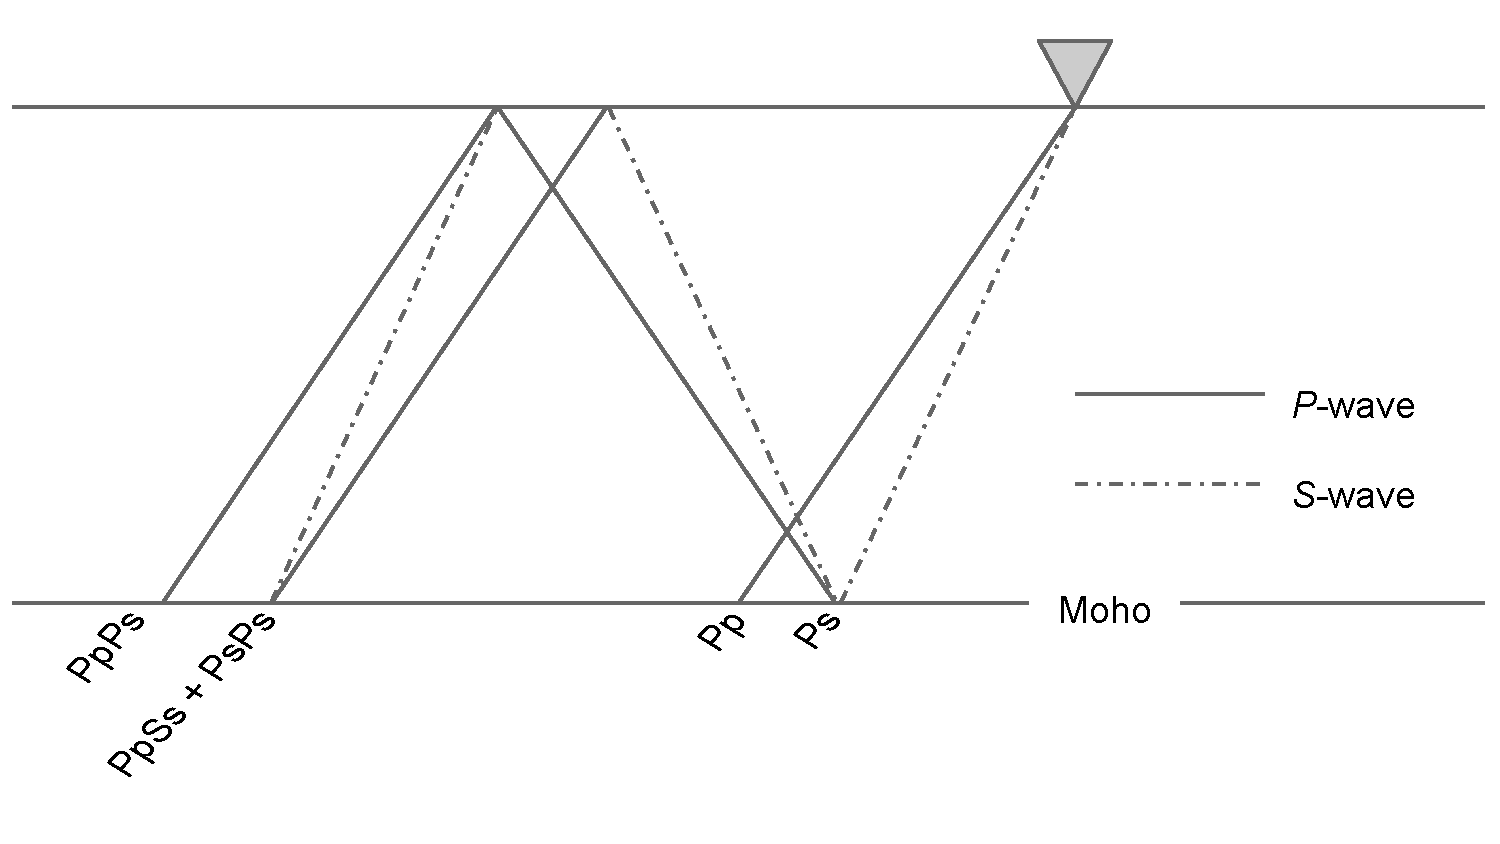
\includegraphics[width=\textwidth]{reflectedPhases}
  \caption{Schematic diagram illustrating geometry of phases for the velocity contrast representing the Moho}
  \label{fig:reflectedPhases}
\end{figure}


  A well tested and widely published method for extracting the ratio, $R=\frac{V_P}{V_S}$, where $V_P$ is P-wave velocity and $V_S$ is S-wave velocity and crustal thickness, or depth to Moho, $H$, is outlined by Zhu and Kanamori [2000], hereafter ZK. This method takes advantage of the differential arrival times between the S-wave reflected phases $Ps$, $PpPs$ $PsPs$, $PpSs$ and $PsSs$ and the direct P-wave arrival $Pp$, Figure ~\ref{fig:reflectedPhases}. Note that $PsPs$ and $PpSs$ have an equal number of $P$ and $S$ phases, and the energy for these two phases arrive simultaneously and are indistinguishable. For a range of slowness values, $p$, the differential arrival times, $t(p)$, trace moveout curves for each phase arrival given by

% Travel time equations
\begin{equation}
t_{Ps}(p_i)=H \left[ \sqrt{ \left(\frac{V_p}{V_s}\right)^2 - p_i^2V_p^2} - \sqrt{1 - p_i^2V_P^2} \right]
\end{equation}

\begin{equation}
t_{Pps}(p_i)=H \left[ \sqrt{ \left(\frac{V_p}{V_s}\right)^2 - p_i^2V_p^2} + \sqrt{1 - p_i^2V_P^2} \right]
\end{equation}

\begin{equation}
t_{Pss}(p_i)= 2H  \sqrt{ \left(\frac{V_p}{V_s}\right)^2 - p_i^2V_p^2}
\end{equation}

where $p_i$ is the slowness for the $i^{th}$ receiver function. Since strong reflected phases occur at sharp velocity contrasts, the Moho, the boundary targeted by ZK, tends to be well represented on most RF's.

  The travel time equations demand an apriori assumption on crustal P-wave velocity, $V_P$, and will trade-off to some degree with crustal thickness $H$. For this study, each station is assigned a $V_P$ values corrisponding to the Crust 2.0 value for the $2^o$ containing cell. In the specific cases where data is being compared to previously published results for quality control, $V_P$  values are chosen to match the values in the published study.

  For a range of candidate models of $R$ and $H$ the RF's are stacked along trial moveout curves. During the stacking procedure each phase is assigned a weight to account for a general trend in the quality of the phases, with direct arrival usually carrying the best signal followed by $PpPs$ and finally $PpSs$. The weights chosen during the stacking are $w1 = 0.5$, $w2 = 0.3$ , $w3 = 0.2$ for the $Ps$, $PpPs$ and $PpSs$ phases respectively. In addition Semblance weighting [Eaton, 2006] is used to reduce the effect of spurious large amplitude noise in the data. The model which stacks the most coherent energy is used to provide the best estimates for the bulk crustal parameters $R$ and $H$ under a given seismic station.


\subsection{Full Gridsearch Method}

\subsection{Vp data}
   Accompanying the processed estimates outlines above are data from controlled source experiments collected and compiled by external sources. The data was compiled by Mooney (personal communication, 2012).

\subsection{Crust 2.0 data}
   Accompanying the processed estimates outlines above are data from controlled source experiments collected and compiled by external sources. The data was compiled by Mooney (personal communication, 2012).


%% -----------------------------------------------%%
\section{Results}

\subsection{Comparisons}
As regional studies exist which utilize similar methods and have corresponding parameter estimates for some of the stations used in this study it is possible to directly compare values to those previously published. A comprehensive study in the Hudson Bay region of the Canadian Shield (Thomson et. al., 2010) uses an approach similar to the Zhu and Kanamori method published estimates for $H$ and $R=\frac{V_P}{V_S}$ for 35 stations. 5 stations with $R$ estimates above 1.8 are removed due to the uncertainty surrounding these high values. There is strong correlation of 0.95 between crustal thickness values for both datasets (Figure~\ref{fig:thompsonCompH}). The velocity ratio data has a lower correlation of 0.5 (Figure~\ref{fig:thompsonCompR}). [Compare this value to uncertainty / deviation in the data? ].

Directly comparing $V_P$ estimates processed with the MB algorithm is not possible as this method has not been employed in publication. However, comparisons can be made to active source records for experiments within close proximity to a given seismic station (Figure~\ref{fig:activeComp}. The correlation between these datasets is 0.235. [This is low, explain here?]. Another method of determining the reliability of estimates is to check the $\frac{V_P}{V_S}$ ratio taken from the Kanamori approach to the $\frac{V_P}{V_S}$ value computed from the MB approach. These values, working with the same data, preprocessed using the same methods and tools should be equal. Selecting only those stations with an error of less than +/-0.05 $R$, 132 stations, we get a correlation of 0.57. Reducing the error tolerance and selecting stations with less than +/-0.01 $R$, leaving 31 of the cleanest stations, we get a correlation coefficient of 0.95.

\begin{figure}
  \centering
    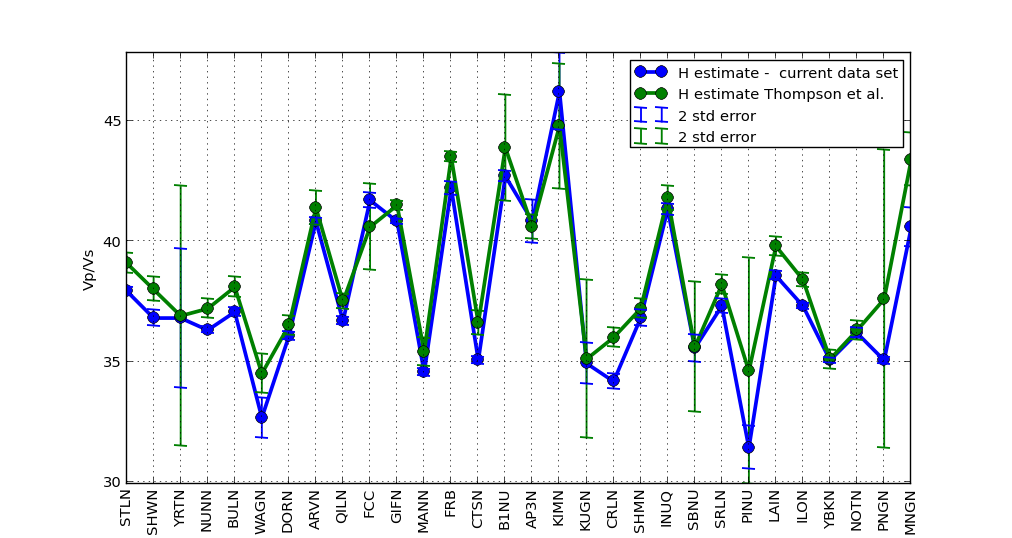
\includegraphics[width=\textwidth]{thompsonComparisonH}
  \caption{Comparison of crustal thickness $H$ data from this study with data from Thomspson et. al. (2010). Data shows a Pearson correlation of 0.95}
  \label{fig:thompsonCompH}
\end{figure}

\begin{figure}
  \centering
    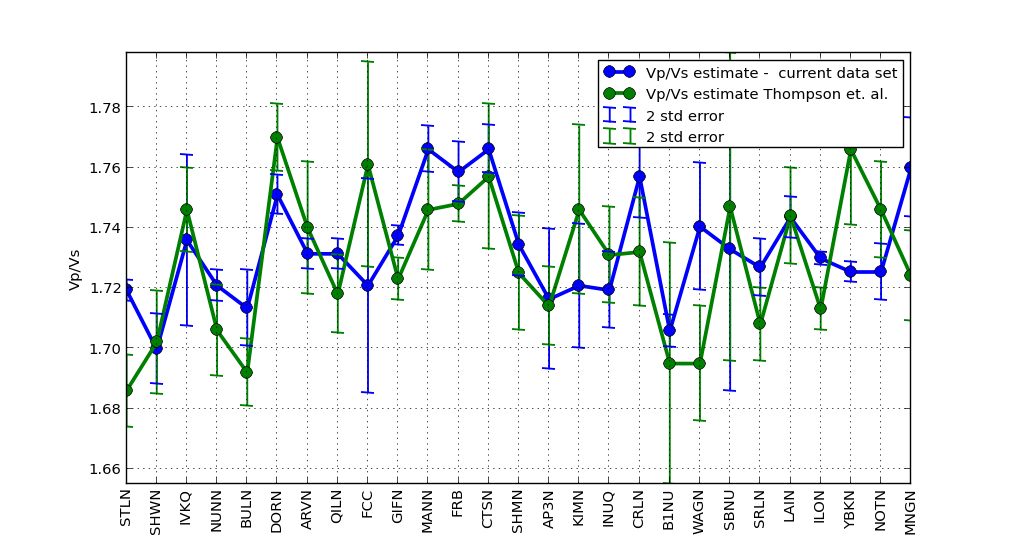
\includegraphics[width=\textwidth]{thompsonComparisonR}
  \caption{Comparison of $V_P / V_R$ data from this study with data from Thomspson et. al. (2010). Data shows a Pearson correlation of 0.5}
  \label{fig:thompsonCompR}
\end{figure}

\begin{figure}
  \centering
    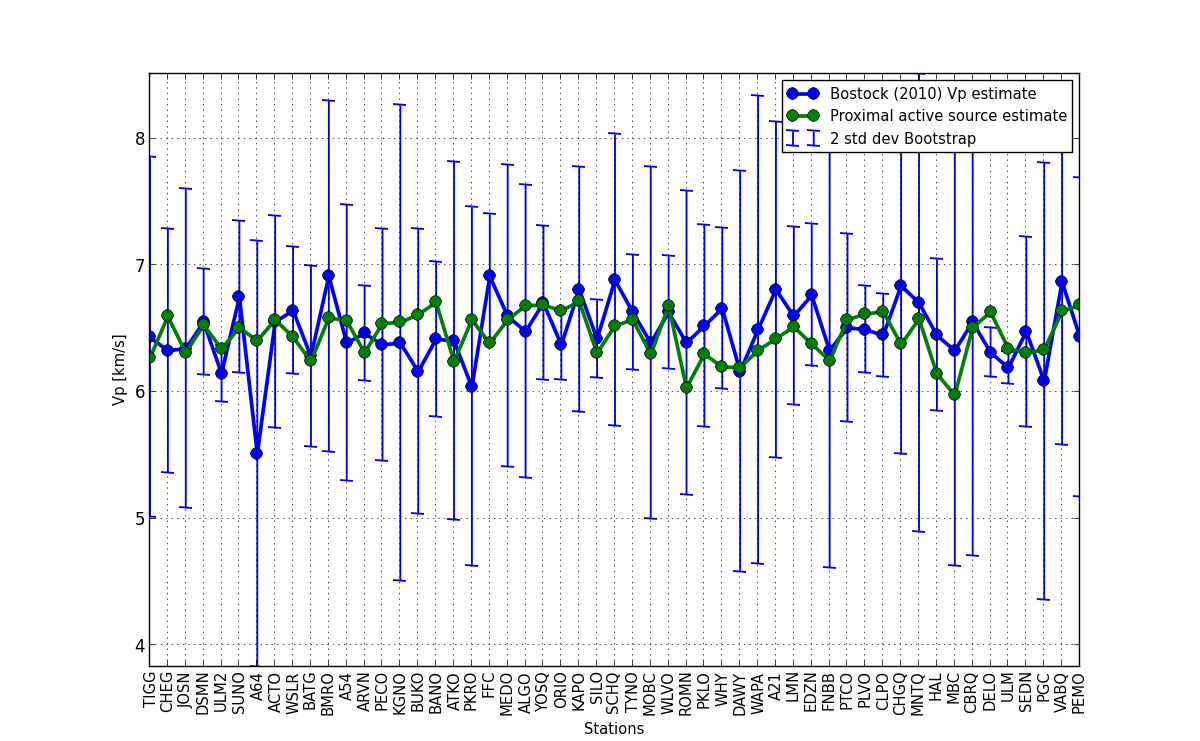
\includegraphics[width=\textwidth]{activeSourceComparison}
  \caption{Comparison of $V_P$ estimates from the MB algorithm with active source $V_P$ recordings. Stations selected if active source experiment locations within 1 degree of latitude / longtitude.}
  \label{fig:activeComp}
\end{figure}

\subsection{Crustal Thickness}
 (MAY NOT INCLUDE)
\begin{itemize}
  \item Jump in crustal thickness over the fault as you go from the Slave to the Rae or Churchill Province.
  \item Trend in Southern Ontario as we move north and up the St Lawrence Seaway.
  \item Appears to be secular variation in the North Eastern Churchill. As we move North and East we have thickening of continental crust.
\end{itemize}

\subsection{Vp/Vs}
\begin{itemize}
  \item reference Figure~\ref{fig:VpVsMap}
  \item For perspective, the value for Quartzite is 1.65 and Basalt is 1.85.
  \item North East of the Slave province, has cluster of low Vp/Vs values in a semi circle of high values.
  \item Appears to be an shift throughout the Superior province from high Vp/Vs in the South to low Vp/Vs in the North East.
  \item Compare to Crust 2.0 overlay (Figure~\ref{fig:VpVsMapCrust}).  Average value for Churchill province Vp/Vs is 1.73 while average value computed from Crust 2.0 is 1.77.
\end{itemize}

\begin{figure}
  \centering
    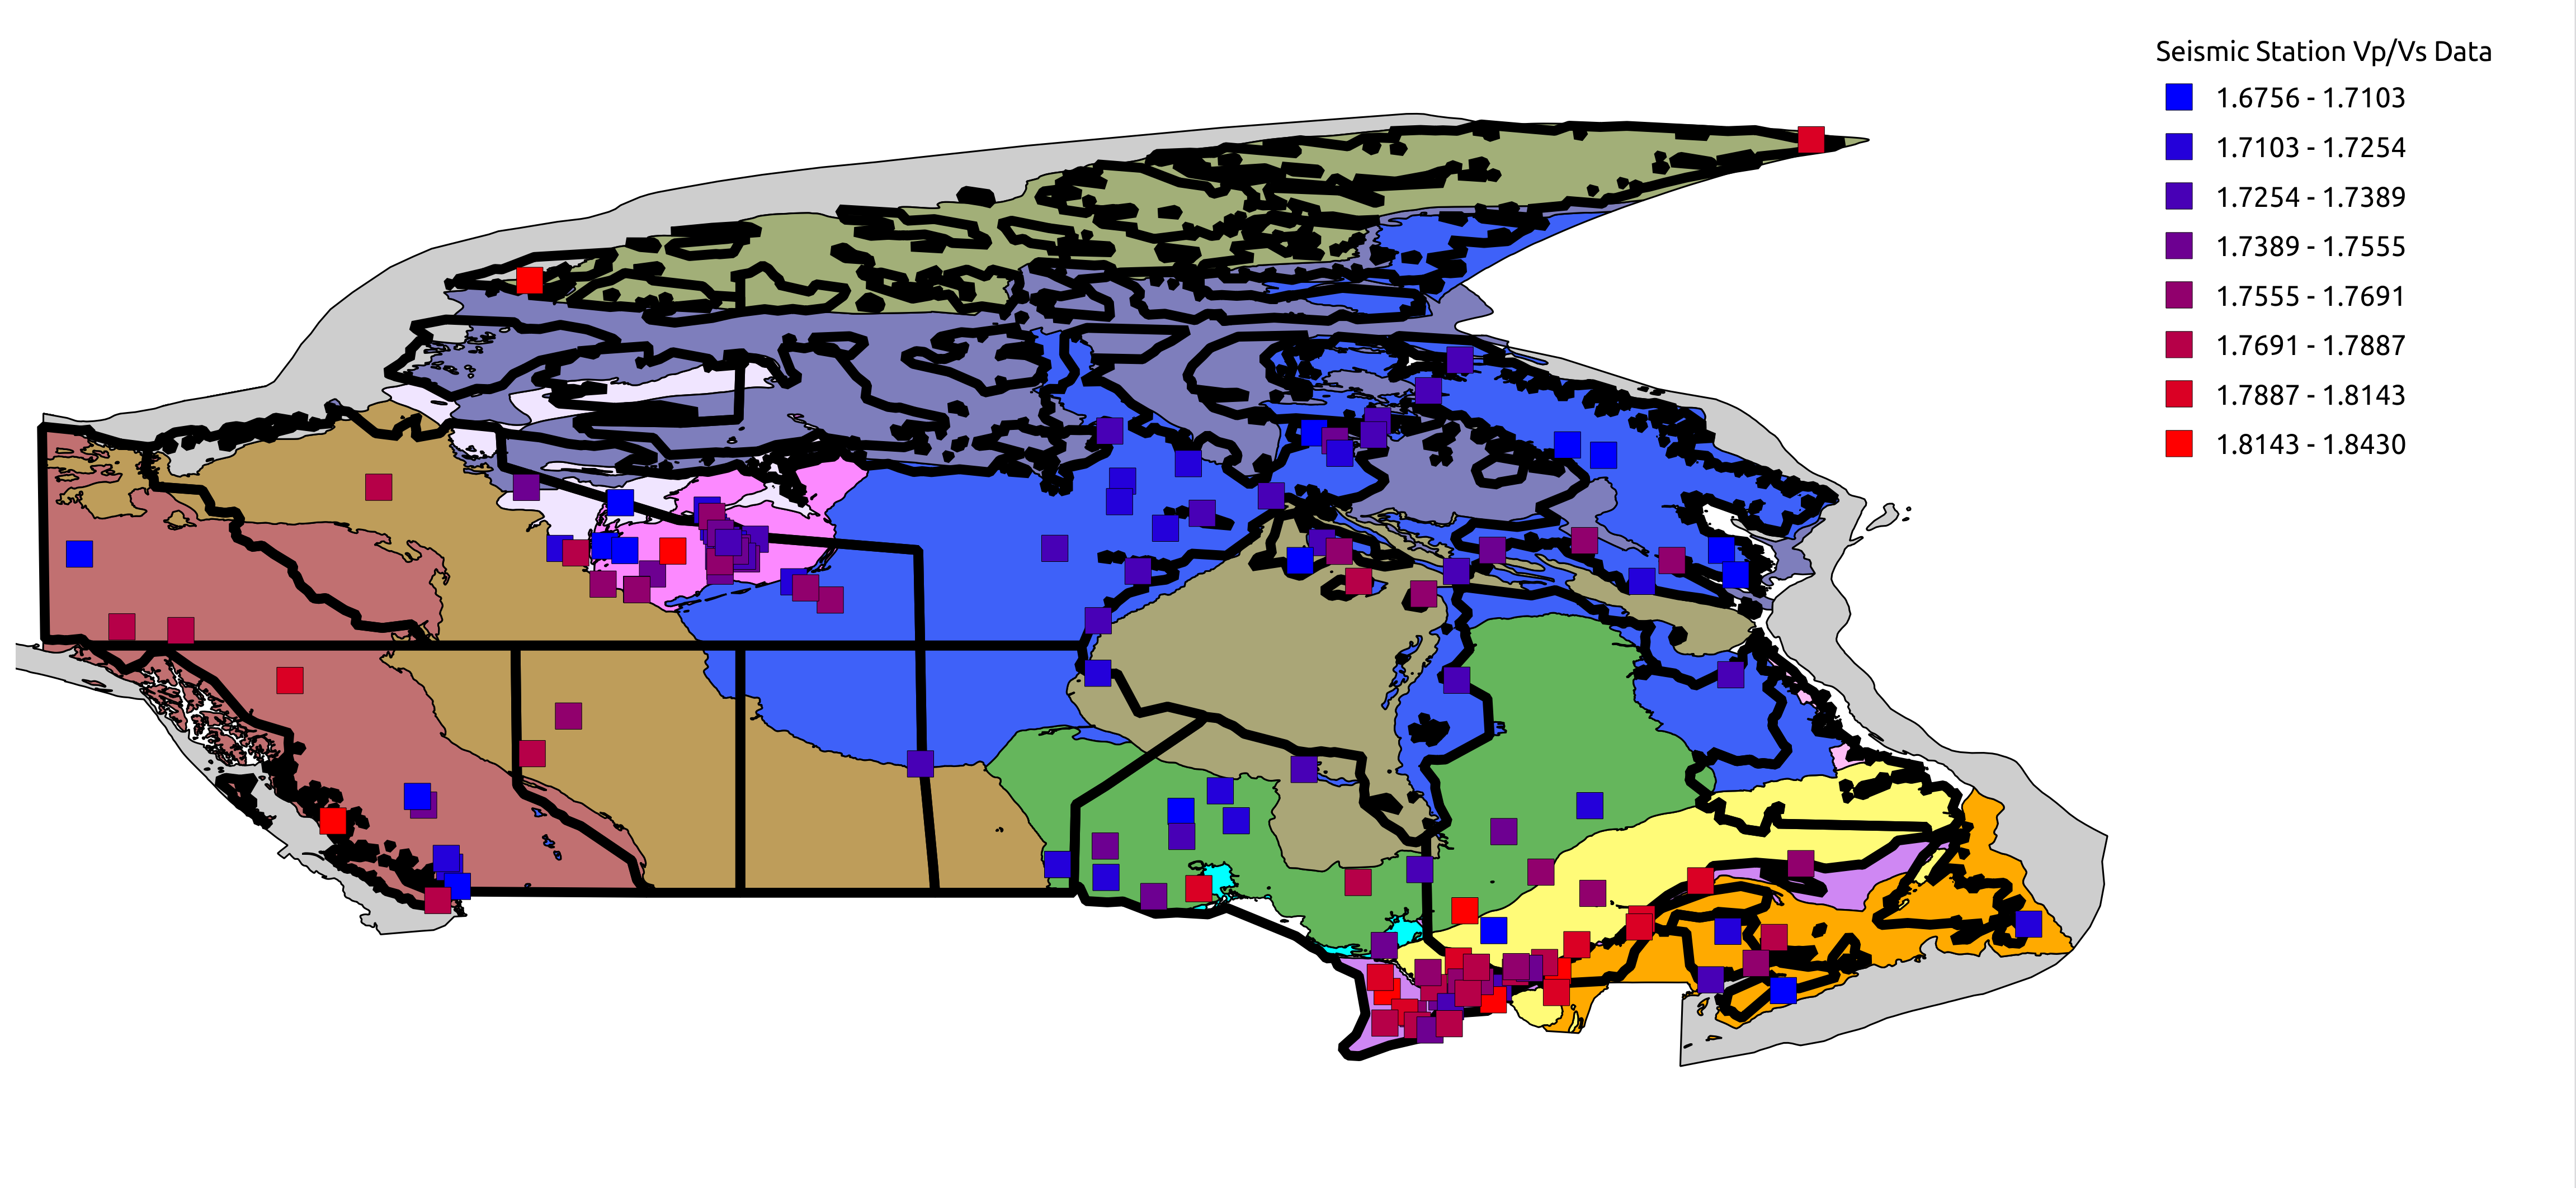
\includegraphics[width=\textwidth]{VpVsMap}
  \caption{}
  \label{fig:VpVsMap}
\end{figure}

\begin{figure}
  \centering
    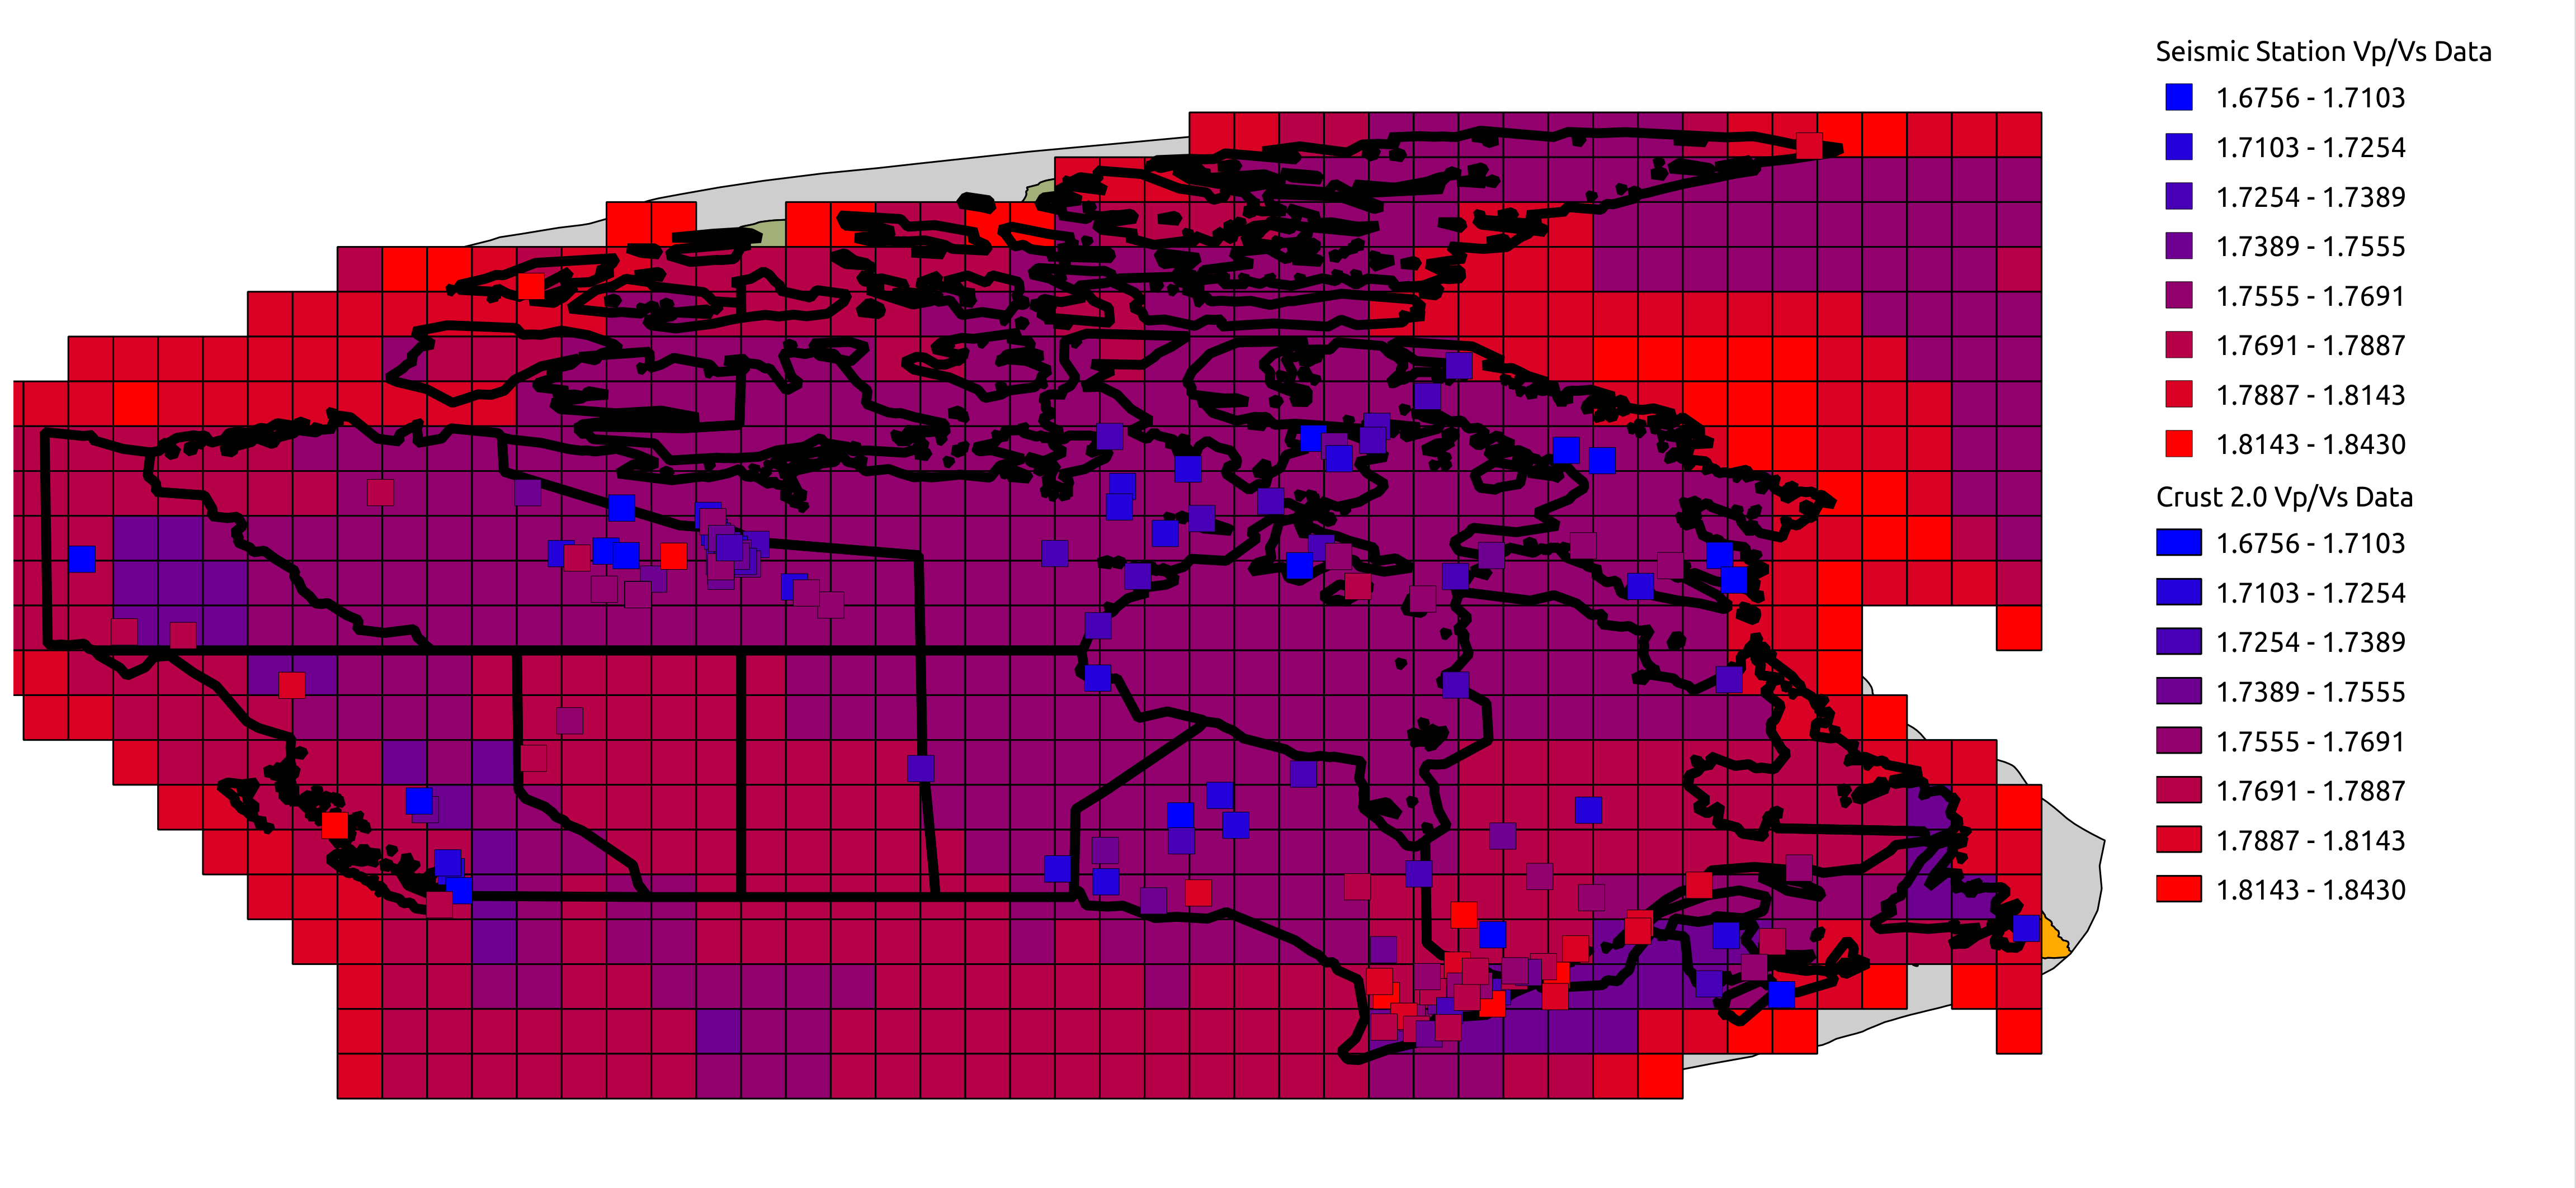
\includegraphics[width=\textwidth]{VpVsMapCrust}
  \caption{}
  \label{fig:VpVsMapCrust}
\end{figure}


%% -----------------------------------------------%%
\section{Discussion}
\subsection{Canada}

  The preliminary interrogation of the data set yields the observation that the bulk Canadian Shield has lower Vp/Vs than anticipated. Previous experiments show crustal averages of 1.77 (Christensen and Mooney, 1995) and 1.78 (Zandt and Ammon, 1995). This compares to computed values of 1.73, 1.74, 1.795 for the Churchill, Superior and Grenville Provinces Vp/Vs ratios respectively.


(MIGHT NOT INCLUDE)  The data bares out earlier results showing Proterozoic crust to have a higher seismic velocity ratio than Archean crust. This follows previous studies on crustal formation that have noted this trend in other regions (Durrheim and Mooney, 1991) . The increased crustal thickness of Proterozoic crust is clearly seen in the active source data while it not visible in data from processed seismic stations.

  Further work on the Bostock-Kumar stacking approach is warranted from a look at the cleanest stations. Before it can be employed in large scale analysis additional denoising methods or alternative deconvolution techniques will need to be investigated to reduce the noise in the data.


\subsection{Slave Province}
<Discussion on Slave Province>

%% -----------------------------------------------%%
\section{Conclusions}
<Conclusions here>

%% ------------------------------------------------------------------------ %%


% AGU does not want a .bib or a .bbl file. Please copy in the contents of your .bbl file here.

\begin{thebibliography}{}


\end{thebibliography}

%Reference citation examples:

%...as shown by \textit{Kilby} [2008].
%...as shown by {\textit  {Lewin}} [1976], {\textit  {Carson}} [1986], {\textit  {Bartholdy and Billi}} [2002], and {\textit  {Rinaldi}} [2003].
%...has been shown [\textit{Kilby et al.}, 2008].
%...has been shown [{\textit  {Lewin}}, 1976; {\textit  {Carson}}, 1986; {\textit  {Bartholdy and Billi}}, 2002; {\textit  {Rinaldi}}, 2003].
%...has been shown [e.g., {\textit  {Lewin}}, 1976; {\textit  {Carson}}, 1986; {\textit  {Bartholdy and Billi}}, 2002; {\textit  {Rinaldi}}, 2003].



%...as shown by \citet{jskilby}.
%...as shown by \citet{lewin76}, \citet{carson86}, \citet{bartoldy02}, and \citet{rinaldi03}.
%...has been shown \citep{jskilbye}.
%...has been shown \citep{lewin76,carson86,bartoldy02,rinaldi03}.
%...has been shown \citep [e.g.,][]{lewin76,carson86,bartoldy02,rinaldi03}.
%
% Please use ONLY \citet and \citep for reference citations.
% DO NOT use other cite commands (e.g., \cite, \citeyear, \nocite, \citealp, etc.).

%% ------------------------------------------------------------------------ %%


\end{document}

%% ------------------------------------------------------------------------ %%


M. G. Bostock, M. R. Kumar, 2010. Bias in seismic estimates of crustal properties, Geophys. J. Int., 182, 403-407.
N. I. Christensen, 1996. Poisson's ratio and crustal seismology, J. Geophys. Res., 101, 3139–3156,
R. J. Durrheim, W. D. Mooney, 1991. Archean and Proterozoic crustal evolution, Geology, 19, 606-609.
W. D. Mooney. 2012. Personal communication. Compiled GSC active source data for the Canada.
D.A. Thompson, I.D. Bastow, G. Helffrich, J-M. Kendall, J. Wookey, D.B. Snyder, D.W. Eaton, 2010. Precambrian crustal evolution: Seismic constraints from the Canadian Shield, Earth and Planetary Science Letters, Volume 297, Issues 3–4, 1 September 2010, Pages 655–666
L. Zhu, H. Kanamori, 2000. Moho depth variation in Southern California from teleseismic receiver functions, J. Geophys Res, 105, 2969-2980.
G. Zandt, C. J. Ammon, 1995. Continental crust composition constrained by measurements of crustal Poisson's ratio, Nature, 374, 152-154.

%
%  SECTION HEADS
%
%% ------------------------------------------------------------------------ %%

ABSTRACT
   It has been suggested that processes driving crustal formation in the Archean and Proterozoic were dissimilar and produced crusts with unique bulk properties and average thicknesses. Existing models based on fractionating mantle composition or evolving mantle convection require accurate estimates of the geological and geophysical properties of crustal provinces to better understand the details of early continental formation (R. Durrheim, W. Mooney, 1991). Fifteen years of publicly accessible teleseismic data from all available Canadian seismic stations are binned in horizontal slowness and deconvolved into receiver functions. We apply a new stacking method (Bostock and Kumar, 2010) to retrieve estimates of bulk crustal velocities (Vp, Vs) and thickness H from these data under the assumption of 1-D structure. Bootstrap error analysis is performed for each station dataset and results are compared to the results produced from alternate methods (Zhu and Kanamori, 2000). Cross-analyzing these results with the mineral and rock seismic property database of Christensen (1996) will afford improved constraints on bulk geological composition of the Canadian landmass. These results will be used to evaluate competing models of early crustal formation.



% Capitalize the first letter of each word (except for
% prepositions, conjunctions, and articles that are
% three or fewer letters).

% AGU follows standard outline style; therefore, there cannot be a section 1 without
% a section 2, or a section 2.3.1 without a section 2.3.2.
% Please make sure your section numbers are balanced.
% ---------------
% Level 1 head
%
% Use the \section{} command to identify level 1 heads;
% type the appropriate head wording between the curly
% brackets, as shown below.
%
%An example:
%\section{Level 1 Head: Introduction}
%
% ---------------
% Level 2 head
%
% Use the \subsection{} command to identify level 2 heads.
%An example:
%\subsection{Level 2 Head}
%
% ---------------
% Level 3 head
%
% Use the \subsubsection{} command to identify level 3 heads
%An example:
%\subsubsection{Level 3 Head}
%
%---------------
% Level 4 head
%
% Use the \subsubsubsection{} command to identify level 3 heads
% An example:
%\subsubsubsection{Level 4 Head} An example.
%
%% ------------------------------------------------------------------------ %%
%
%  IN-TEXT LISTS
%
%% ------------------------------------------------------------------------ %%
%
% Do not use bulleted lists; enumerated lists are okay.
% \begin{enumerate}
% \item
% \item
% \item
% \end{enumerate}
%
%% ------------------------------------------------------------------------ %%
%
%  EQUATIONS
%
%% ------------------------------------------------------------------------ %%

% Single-line equations are centered.
% Equation arrays will appear left-aligned.

Math coded inside display math mode \[ ...\]
 will not be numbered, e.g.,:
 \[ x^2=y^2 + z^2\]

 Math coded inside \begin{equation} and \end{equation} will
 be automatically numbered, e.g.,:
 \begin{equation}
 x^2=y^2 + z^2
 \end{equation}

% IF YOU HAVE MULTI-LINE EQUATIONS, PLEASE
% BREAK THE EQUATIONS INTO TWO OR MORE LINES
% OF SINGLE COLUMN WIDTH (20 pc, 8.3 cm)
% using double backslashes (\\).

% To create multiline equations, use the
% \begin{eqnarray} and \end{eqnarray} environment
% as demonstrated below.
\begin{eqnarray}
  x_{1} & = & (x - x_{0}) \cos \Theta \nonumber \\
        && + (y - y_{0}) \sin \Theta  \nonumber \\
  y_{1} & = & -(x - x_{0}) \sin \Theta \nonumber \\
        && + (y - y_{0}) \cos \Theta.
\end{eqnarray}

%If you don't want an equation number, use the star form:
%\begin{eqnarray*}...\end{eqnarray*}

% Break each line at a sign of operation
% (+, -, etc.) if possible, with the sign of operation
% on the new line.

% Indent second and subsequent lines to align with
% the first character following the equal sign on the
% first line.

% Use an \hspace{} command to insert horizontal space
% into your equation if necessary. Place an appropriate
% unit of measure between the curly braces, e.g.
% \hspace{1in}; you may have to experiment to achieve
% the correct amount of space.


%% ------------------------------------------------------------------------ %%
%
%  EQUATION NUMBERING: COUNTER
%
%% ------------------------------------------------------------------------ %%

% You may change equation numbering by resetting
% the equation counter or by explicitly numbering
% an equation.

% To explicitly number an equation, type \eqnum{}
% (with the desired number between the brackets)
% after the \begin{equation} or \begin{eqnarray}
% command.  The \eqnum{} command will affect only
% the equation it appears with; LaTeX will number
% any equations appearing later in the manuscript
% according to the equation counter.
%

% If you have a multiline equation that needs only
% one equation number, use a \nonumber command in
% front of the double backslashes (\\) as shown in
% the multiline equation above.

%% ------------------------------------------------------------------------ %%
%
%  LANDSCAPE/SIDEWAYS FIGURE AND TABLE EXAMPLES
%
%% ------------------------------------------------------------------------ %%
%
% For figures, add \usepackage{lscape} to the file and the landscape.sty style file
% to the paper folder.
%
% \begin{figure*}[p]
% \begin{landscapefigure*}
% Illustration here.
% \caption{caption here}
% \end{landscapefigure*}
% \end{figure*}
%
% For tables, add \usepackage{rotating} to the paper and add the rotating.sty file to the folder.
%
% AGU prefers the use of {sidewaystable} over {landscapetable} as it causes fewer problems.
%
% \begin{sidewaystable}
% \caption{}
% \begin{tabular}
% Table layout here.
% \end{tabular}
% \end{sidewaystable}
%
%
